% Appendix A. Instalacion de gnuradio
%==========================================================================

\chapter{Instalaci\'on del ambiente de desarrollo}
\label{AppA}

El desarrollo de aplicaciones basadas en \emph{GNURadio} en el ambiente Linux es
m\'as sencillo y m�\'as vers\'atil ya que la mayor\'ia de las librer\'ias
externas de las que depende esta herramienta fueron desarrolladas para Linux.
Aunque \emph{GNURadio} proporciona soporte parcial/total para otros sistemas
operativos como \emph{Windows} y \emph{Mac OSX}, el experimento se realizo en el
sistema operativo \emph{Ubuntu}, que es una distribuci\'on del sistema operativo
Linux basado en una distribuci\'on llamada \emph{Debian}. Se opto por esta
versi\'on de Linux ya que es la m\'as amigable y f\'acil de usar pero
principalmente se escogi\'o por su habilidad de poder ser instalado dentro de
\emph{Windows} como una aplicaci\'on normal. Esto evita tener que hacer una
partici\'on separada para instalar el sistema operativo. Si se desea quitar es
solo cuestion de ir al panel de control de \emph{Windows} y desinstalar
\emph{Ubuntu}. Estar\'a en la lista de aplicaciones instaladas.

Para poder llevar a cabo este procedimiento se utilizo un programa especial
llamado \emph{Wubi} \cite{russo}. Esta aplicaci\'on instala el sistema operativo
dentro de un solo archivo y agrega una nueva opci\'on al men\'u de arranque de
la PC para poder seleccionarlo aparte del sistema operativo primario. Cuando se
ejecuta el programa \emph{Wubi}, se deben especificar las opciones que se
muestran en la figura \ref{fig:wubi}. Se puede dejar el tama\~no del archivo
generado en su opci\'on default pero se recomienda que m\'inimo se le asigne 10 gigabytes para
tener suficiente espacio para la instalaci\'on de librer\'ias que se vallan a
requerir para la aplicaci\'on, aunque si el usuario desea instalar otras
aplicaciones que no son parte de este tema entonces ser\'a necesario incrementar
este valor. Se debe especificar un nombre de usuario y la clave para esta cuenta
ya que esta ser\'a la cuenta principal donde se realizara todo el trabajo.
Posteriormente una vez terminando la instalaci\'on se pueden crear m\'as
usuarios si uno lo desea.

\begin{figure}[hpt]
\centering
	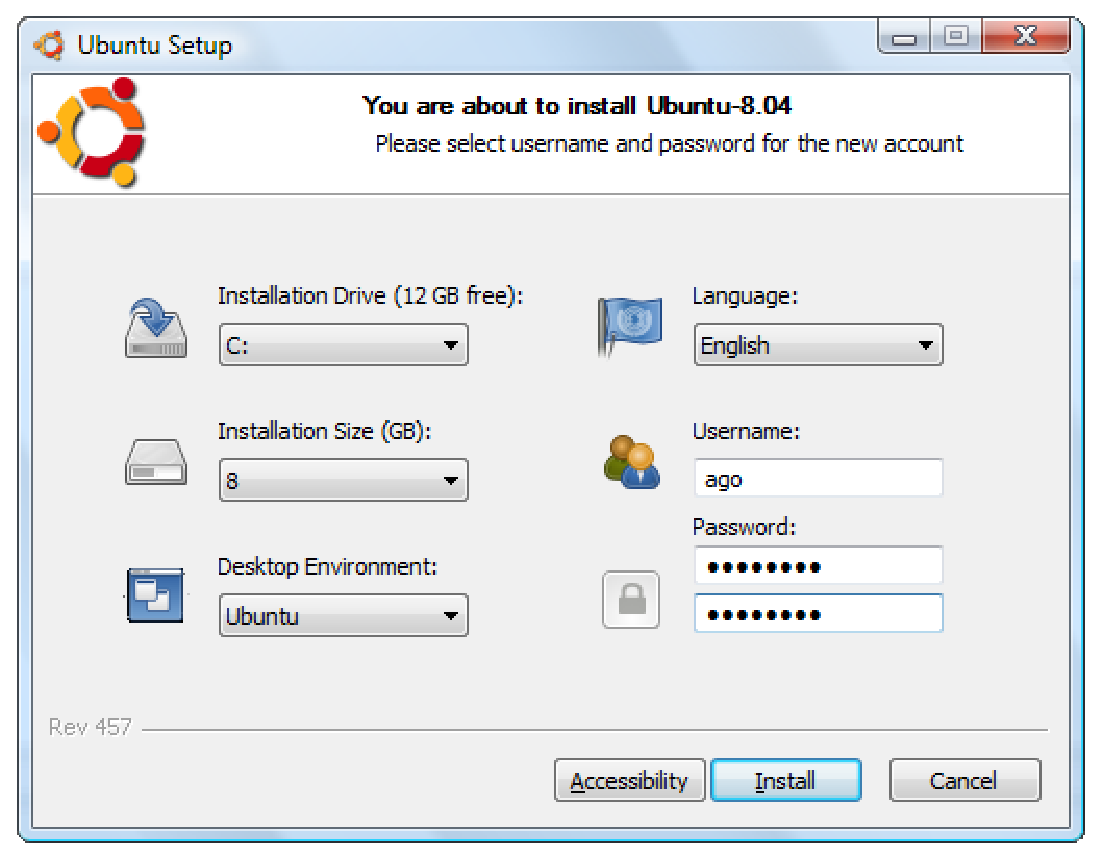
\includegraphics[scale=0.5]{figs/wubi}
	\caption{Opciones del instalador \emph{Wubi}}
	\label{fig:wubi}
\end{figure}

Una vez que se halla especificado las opciones anteriores se puede entonces
iniciar con la instalaci\'on. \emph{Wubi} comenzar\'a a bajar de internet la
imagen del DVD correspondiente a la distribuci�n de \emph{Ubuntu} que se
especifico.

Cabe mencionar que la instalaci\'on puede ser de 32 o 64 bits, dependiendo del
tipo de instalaci\'on de \emph{Windows} donde se va instalar \emph{Ubuntu}. Si
el sistema operativo principal es de 32 bits entonces la instalaci\'on tambi\'en
ser\'a de 32 bits. Esto se debe tener presente cuando se inicie la instalaci\'on
de \emph{GNURadio} ya que las librer\'ias de las cuales depende vienen en
versiones de 32 y 64 bits.

La imagen mide aproximadamente 700MB. Cuando termine de bajarlo la aplicaci\'on
comenzar\'a a crear el archivo del sistema operativo y agregara la opci\'on para
seleccionarlo en el men\'u de arranque como se muestra en la figura
\ref{fig:bootmenu}. Una vez terminado este procedimiento la aplicaci\'on le
pedir\'a al usuario que reinicie la PC. Ahora necesitamos seleccionar la nueva opci�n del men\'u de arranque para
poder ingresar al sistema operativo \emph{Ubuntu}. El usuario no tiene que hacer
nada por su parte ya que la instalaci\'on del sistema operativo se lleva a cabo
de modo autom\'atico. Al terminar se le presentara al usuario que ingrese el
nombre de la cuenta y la clave. Esta es la que se especifico en el instalador
\emph{Wubi}. Realizando esto nos encontraremos en el escritorio \emph{GNOME} (o
\emph{KDE} si se especific\'o otra distribuci\'on como \emph{Kubuntu}) como se
muestra en la figura \ref{fig:desktop}.

\begin{figure}[htp]
\centering
	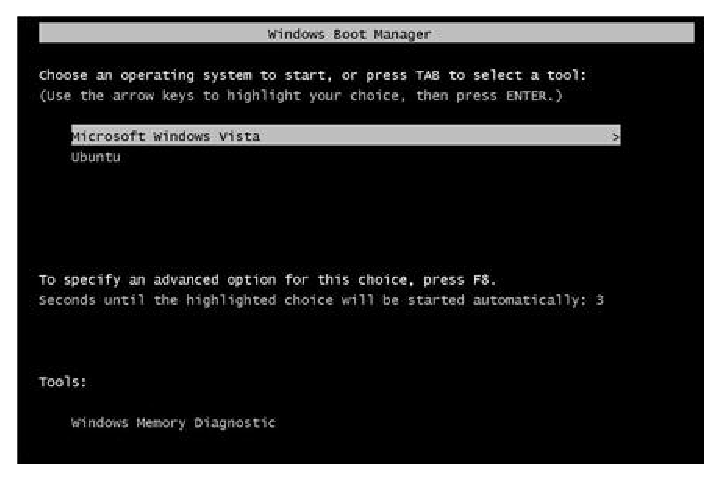
\includegraphics[scale=0.8]{figs/boot}
	\caption{Men\'u de arranque con la opci\'on de \emph{Ubuntu}}
	\label{fig:bootmenu}
\end{figure}

\begin{figure}[htp]
\centering
	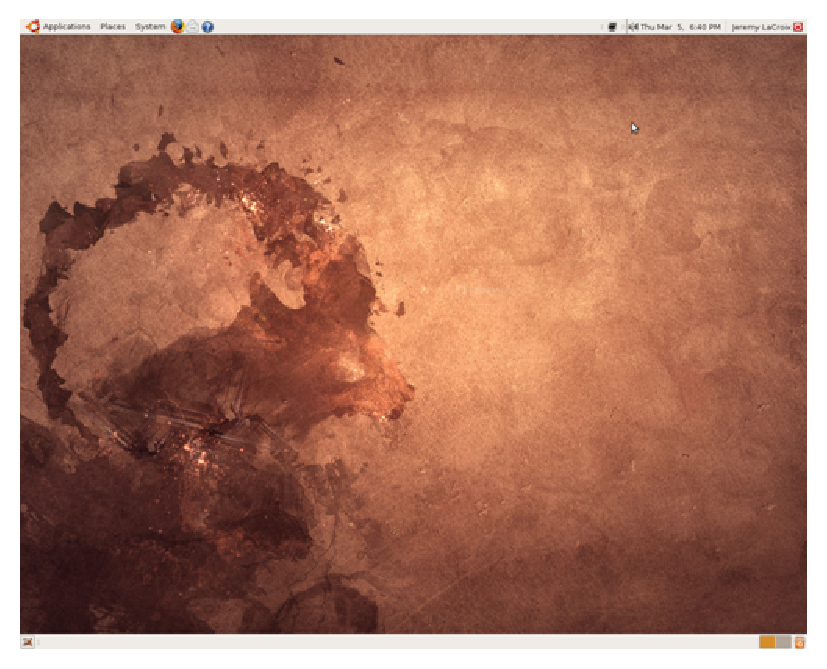
\includegraphics[scale=0.7]{figs/desk}
	\caption{Escritorio \emph{GNOME} de la distribuci\'on \emph{Ubuntu}}
	\label{fig:desktop}
\end{figure}

El siguiente paso es instalar \emph{GNURadio} y sus dependencias. Todas
las dependencias se pueden conseguir utilizando el sistema de instalaci\'on de
software de \emph{Ubuntu} lo cual hace la instalaci\'on m\'as f\'acil. En
versiones anteriores a 9.04 uno ten\'ia que bajar manual mente el c\'odigo
fuente de varias p\'aginas de internet y compilarlo manualmente. Utilizando el
sistema Synaptic del sistema operativo se deben instalar las dependencias que se
especifican en la tabla \ref{tbl:radioreqs}.

\begin{table}[htp]
\begin{center}
	\begin{tabular}{|p{6cm}|p{7.5cm}|}
		\hline
		Tipo & Elementos \\
		\hline
		Herramientas de desarrollo que se requieren para compilar el c\'odigo fuente.
		& 
		\begin{itemize}
		  \item g++
		  \item subversion
		  \item make
		  \item autoconf, automake, libtool
		  \item sdcc
		  \item guile
		  \item ccache
		  \item SWIG 1.3.31 o mayor
		  \item git
		\end{itemize} \\
		\hline
		Librer\'ias requeridas para compilaci\'on y funcionamiento de los ejecutables.
		&
		\begin{itemize}
		  \item python-dev
		  \item FFTW 3.X (fftw3, fftw3-dev)
		  \item CppUnit (libcppunit y libcppunit-dev)
		  \item Boost 1.35 o mayor
		  \item libusb y libusb-dev
		  \item wxWidgets (wx-common y python-wxgtk)
		  \item python-numpy
		  \item ALSA (alsa-base, libasound2, libasound2-dev)
		  \item Qt4
		  \item SDL (libsdl-dev)
		  \item GSL GNU Scientific Library (libgsl0-dev) 1.10 o mayor
		\end{itemize}\\
		\hline
		Elementos opcionales &
		\begin{itemize}
		  \item QWT 5.0 o mayor
		  \item QWT Plot3d para QT4
		  \item Python-scipy, python-matplotlib, python-tk
		  \item Doxygen
		  \item Octave
		\end{itemize}\\
		\hline
	\end{tabular}
	\vspace{0.5in}
	\caption{Dependencias requeridas para la instalaci\'on de \emph{GNURadio}}
	\label{tbl:radioreqs}
\end{center}
\end{table}

La \'unica librer\'ia que se recomienda que se instale manualmente es
\emph{Boost} ya que la m\'as reciente es la versi\'un 1.43 y ofrece muchas
mejoras contra la versi�n 1.38 de Ubuntu. Para instalarla es cuesti\'on de bajar
el c\'odigo fuente de la p\'agina \url{www.Boost.org} y seguir los siguientes
pasos:

\begin{enumerate}
  \item Descargar el c\'odigo fuente a un lugar adecuado, abrir una consola e
  ir al directorio donde se descargo el archivo.
  \item Descomprimir el archivo con el siguiente comando:\\
  \verb|tar xfz boost_1_43_0.tar.gz|
  \item Entrar al directorio nuevo que se cre\'o al descomprimir el archivo y
  ejecutar el siguiente comando: \verb|./bootstrap.sh|
  \item Ejecutar el siguiente comando: \verb|sudo ./bjam install| Se debe
  proporcionar la clave de la cuenta que estamos usando ya que la instalaci\'on
  requiere privilegios de administrador.
\end{enumerate}

La compilaci\'on e instalaci\'on puede durar entre 20 y 30 minutos dependiendo
de la velocidad de la PC. Este procedimiento compilara e instalara todas las
librer\'ias que forman parte del conjunto de \emph{Boost}. Este proceso se puede
controlar m\'as detalladamente para que \'unicamente instale un subconjunto de
librer\'ias y as� reducir m\'as el tiempo de instalaci\'on ya que
\emph{GNURadio} no utiliza todo el conjunto completo.

Despu\'es de instalar \emph{Boost} se necesita utilizar el sistema
\emph{Synaptic} para instalar el resto de las dependencias como se menciono
anteriormente. Esta herramienta se encuentra en el men\'u
\emph{System\ding{219}Administration\ding{219}Synaptic Package Manager} y se
muestra en la figura \ref{fig:synaptic}. En la caja de texto que dice search se
puede escribir el nombre de las dependencias para que la b\'usqueda sea m\'as r\'apida. Cada que se
seleccione una el administrador de paquetes puede notificarle que es necesario
instalar otras sub-dependencias. Esto es autom\'atico y el usuario no tiene que
seleccionarlas manualmente.

\begin{figure}
\centering
	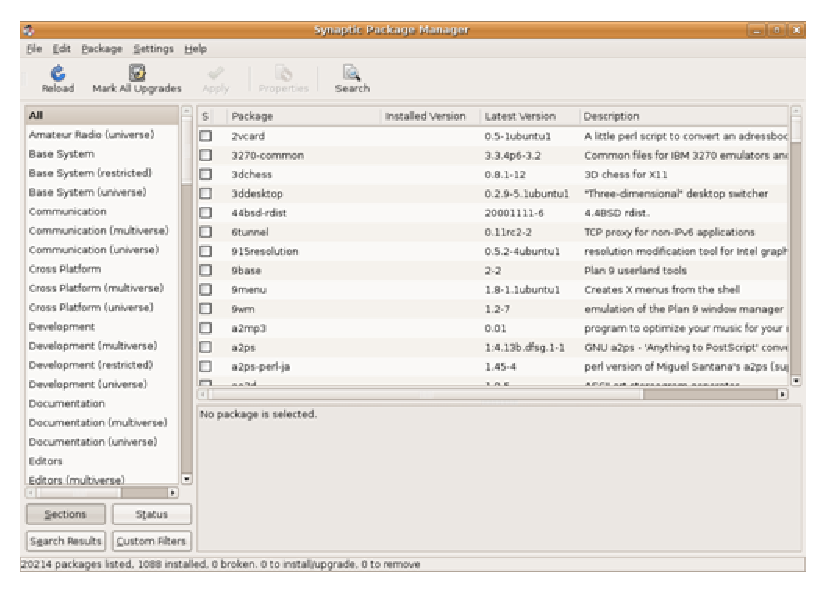
\includegraphics[scale=0.7]{figs/synaptic}
	\caption{Administrador de software Synaptic}
	\label{fig:synaptic}
\end{figure}

Para llevar a cabo este procedimiento se deben seguir los siguientes pasos:

\begin{enumerate}
  \item Abrir una consola e ir a un directorio adecuado para descargar el
  c\'odigo fuente.
  \item Ejecutar el siguiente comando para obtener el codigo fuente de GIT:\\
  \verb|git clone http://gnuradio.org/git/gnuradio.git|. Esto crear\'a un nuevo
  directorio llamado \emph{gnuradio}.
  \item Entrar al nuevo directorio y ejecutar el siguiente comando:\\
  \verb|./bootstrap|
  \item Ejecutar el siguiente comando para configurar la instalaci\'on:\\
  \verb|./configure|
  \item Iniciar la compilaci\'on con el siguiente comando: \verb|make|
  \item Realizar una serie de pruebas para asegurar que la compilaci\'on fue
  exitosa:\\
  \verb|make check|
  \item Instalar \emph{GNURadio}: \verb|sudo make install|
\end{enumerate}

De acuerdo a la documentaci\'on de \emph{GNURadio}, antes de realizar las
pruebas que verifican la compilaci\'on es necesario ejecutar la siguiente serie
de comandos:

\begin{enumerate}
  \item Copiar el archivo \emph{ld.so.conf} a un directorio temporal para
  modificarlo:\\
  \verb|cp /etc/ld.so.conf /tmp/ld.so.conf|
  \item Agregar la ruta donde est\'an instaladas las librer\'ias:\\
  \verb|echo /usr/local/lib >> /tmp/ld.so.conf|
  \item Borrar el archivo temporal y mover el nuevo a su lugar orignal:\\
  \verb|mv /tmp/ld.so.conf /etc/ld.so.conf|
  \item Ejecutar el siguiente comando para aplicar los cambios:\\
  \verb|sudo ldconfig|
\end{enumerate}

La raz\'on del procedimiento anterior es que \emph{Ubuntu} utiliza una
implementaci\'on diferente de la herramienta \emph{libtool} y si la ruta de las
librer\'ias no est\'a especificada en el archivo de configuraci\'on las pruebas
de \emph{GNURadio} van a fallar con errores de que no se encuentran dichas
librer\'ias \cite{radio}.


Para el uso \'optimo del USRP es necesario realizar una modificaci\'on en el
servicio \emph{udev} ya que \'unicamente permite acceso directo del dispositivo
a cuentas con privilegios de administrador. Esto quiere decir que cada que
necesitemos ejecutar alg\'un programa que utilice el puerto USB va ver necesidad
de elevar el ejecutable con el comando sudo. Para evitar hacer esto cada que se
ejecute la aplicaci\'on del usuario se aplican los siguientes pasos:

\begin{enumerate}
  \item Crear un nuevo grupo de usuarios:\\
  \verb|sudo addgroup usrp|
  \item Anexar la cuenta de usuario que se est\'a utilizando a este nuevo
  grupo:\\
  \verb|sudo usermod �G usrp �a <CUENTA_DE_USUARIO>|
  \item Crear un archivo temporal con las instrucciones que \emph{udev} necesita
  para agregar este nuevo grupo a los que est\'an permitidos acceder al puerto
  USB:\\
  \verb|echo �ACTION==�add�, BUS==�usb�, SYSFS{idVendor}==�fffe�,|\\
  \verb|SYSFS{idProduct}==�0002�, GROUP:=�usrp�, MODE:=�0660�� > tmpfile|
  \item Modificar los atributos de este archivo para que sea propiedad de root:\\
  \verb|sudo chown root.root tmpfile|
  \item Mover el archivo temporal al directorio de reglas de \emph{udev}:\\
  \verb|sudo mv tmpfile /etc/udev/rules.d/10-usrp.rules|
\end{enumerate}

Es posible aplicar los cambios al ejecutar el siguiente comando: 
\emph{sudo udevadm control�reload-rules}. Si esto no funciona entonces se necesita reiniciar la PC
para que los cambios tengan efecto.
